\documentclass[10pt,a4paper]{article}

\usepackage{tocloft}
\usepackage{commons/course}
\usepackage{listings}
\usepackage{xcolor}
\usepackage{geometry}
\geometry{margin=1in}
\usepackage{booktabs}
\usepackage[utf8]{inputenc}

% Define colors for syntax highlighting
\definecolor{keywordstyle}{rgb}{0.0, 0.4, 0.8} % A bluer shade
\definecolor{stringstyle}{rgb}{0.9, 0.17, 0.31} % amaranth
\definecolor{commentstyle}{rgb}{0.1, 0.6, 0.2} % green
\definecolor{numberstyle}{rgb}{0.4, 0.4, 0.4} % gray
\definecolor{backgroundcolor}{rgb}{0.94, 0.97, 1.0} % aliceblue

% Define the Python-like language for syntax highlighting
\lstdefinelanguage{PythonLike}{
	morekeywords={mov, add, sub, cmp, jmp , lw , addi,sw,bne},
	sensitive=false,
	morecomment=[l]{;},
	morestring=[b]",
}

% Set the style for Python-like code
\lstset{
	language=PythonLike,
	basicstyle=\ttfamily\small,
	keywordstyle=\color{keywordstyle},
	stringstyle=\color{stringstyle},
	commentstyle=\color{commentstyle},
	numbers=left,
	numberstyle=\tiny\color{numberstyle},
	stepnumber=1,
	numbersep=5pt,
	keepspaces=true,
	tabsize=4,
	showspaces=false,
	showstringspaces=false,
	showtabs=false,
	breaklines=true,
	breakatwhitespace=false,
	frame=single,
	backgroundcolor=\color{backgroundcolor},
}

\newlistof{listofproblems}{lop}{\normalsize فهرست مسائل}
\newcommand{\addproblem}[1]{\addcontentsline{lop}{listofproblems}{\protect\numberline{}#1}}


\begin{document}


\سربرگ{تمرین دوم}{}{پاسخ‌دهنده: معین آعلی - 401105561}{استاد: امیرمهدی صادق‌زاده}


\listoflistofproblems

\bigskip
\bigskip
\hrule\pagebreak

\مسئله{‌}
\subsectionaddtolist{آ}

کل بسته دارای 3000 بایت است و هدر ما 20 بایت، پس دیتا 2980 بایت است. از طرفی می‌دانیم که هر فرگمنت 1480 بایت داده منتقل می‌کند. پس حداقل به 3 فرگمنت برای این کار نیاز داریم.

\[
3 > \frac{2980}{1480} > 2
\]

\subsectionaddtolist{ب}


از بین روترهای A و B و C روتر C بیشترین پیشوند مشترک را دارد و بسته به آن روتر فرستاده می‌شود. همچنین داخل شبکه روتر D قرار ندارد و اصلا مچ نمیشود.

\subsectionaddtolist{ج}

\begin{itemize}
	\item \textbf{درست.}
	پروتوکل $IPv6$ با داشتن فضای آدرس‌دهی بسیار بزرگ، نیاز به ترجمه آدرس شبکه که در $IPv4$ برای جبران کمبود آدرس‌ها استفاده می‌شود را کاهش می‌دهد.
	\item \textbf{درست.}
	تونلینگ به عنوان روشی برای ارسال بسته‌های یک پروتکل داخل پروتکل دیگر استفاده می‌شود که در VPN ها و همچنین برای عبور $IPv6$ روی زیرساخت $IPv4$ کاربرد دارد.
\end{itemize}



\subsectionaddtolist{د}


\begin{itemize}
	\item \textbf{ضعف.}
چون NAT باعث می‌شود دستگاه‌ها در داخل شبکه محلی آدرس‌های خصوصی داشته باشند و همه آنها پشت یک آدرس عمومی مشترک مخفی شوند، این موضوع مدیریت و شناسایی دستگاه‌ها را پیچیده‌تر می‌کند.
	\item \textbf{ضعف.}
زیرا NAT نیاز به پردازش اضافه برای ترجمه آدرس‌ها دارد که ممکن است تاخیر کمی ایجاد کند و همچنین پنهان کردن آدرس‌های واقعی باعث می‌شود عیب‌یابی شبکه دشوارتر شود.

\end{itemize}


\pagebreak


\مسئله{‌}
\begin{itemize}
    \item  UDP ساده‌تر از TCP است (بدون کنترل اتصال، شماره‌گذاری بسته‌ها یا کنترل ازدحام)، پس سرعت انتقال داده بیشتر می‌شود.
    \item نیاز به حداقل تأخیر در برنامه‌هایی که نیاز دارند داده خیلی سریع برسد. مثل تماس صوتی یا لایو استریم.
    تأخیر کم مهم‌تر از تحویل تضمینی همه داده‌ها است. TCP به خاطر مکانیسم‌های تصحیح خطا، تأخیر بیشتری دارد که برای این نوع اپلیکیشن‌ها مناسب نیست.
    \item این اپلیکیشن‌ها طوری طراحی شده‌اند که حتی اگر برخی بسته‌ها از دست برود، همچنان به کار ادامه می‌دهند (مثلاً در تماس صوتی، یک کلمه گم شود ولی مکالمه قطع نشود).
\end{itemize}

برای مثال می‌توان به برنامه تماس تصویری و تماس صوتی و بازی‌های انلاین اشاره کرد.
\pagebreak



\مسئله{‌}
زمان مورد نیاز برای جست‌وجوی DNS به این صورت است:

\setLTR
$
RTT_1 + RTT_2 + RTT_3 + RTT_4 = 250 + 150 + 100 + 50 = 500ms
$
\setRTL


\subsectionaddtolist{الف}{

در این حالت به ازای هر فایل رو کانکشن TCP تشکیل داده و فایل را دریافت میکنیم. به ازای هر فایل هم به 2 RTT نیاز داریم. یکی برای تشکیل کانکشن TCP و یکی هم برای دریافت فایل. پس در مجموع:

\setLTR
$
DNS + 3 \times (2 \times RTT_0) = 500 + 6 \times 300 = 2300ms
$
\setRTL

}

\subsectionaddtolist{ب}{
	
	در این حالت هر سه فایل موازی و با یک کانکشن مخصوص به خود دریافت میشوند، پس برای هرسه فایل نیاز به 2 RTT داریم. زمان DNS هم که همچنان نیاز است، پس:
	
	\setLTR
	$
	DNS + (RTT_0 + RTT_0) = 300 + 300 + 500 = 1100ms
	$
	\setRTL
	
	
}

\subsectionaddtolist{ج}{
	در این حالت فقط 1 کانکشن TCP داریم که همه فایل ها یکی یکی از همین دانلود میشوند.  پس یک DNS داریم و یک RTT برای اتصال TCP و به ازای هر فایل هم یک  RTT . پس:
	
	
		\setLTR
	$
	DNS + (RTT_0 + RTT_0 + RTT_0 + RTT_0) = 500 + 1200 = 1700ms
	$
	\setRTL
}




\pagebreak


\مسئله{‌}
پهنای باند اختصاص داده شده به هر اتصال:

\setLTR
$r = \frac{500}{N} bps$
\setRTL

زمان ارسال یک بسته کنترلی:

\setLTR
$t_{ctrl} = \frac{500bit}{\frac{500}{N} bps} = N s$
\setRTL

زمان ارسال یک بسته داده کوچک:

\setLTR
$t_{100k} = \frac{100000}{\frac{500}{N}} = 200N s $
\setRTL

زمان ارسال یک بسته داده بزرگ:

\setLTR
$t_{300k} = \frac{300000}{\frac{500}{N}} = 600N s $
\setRTL

\subsectionaddtolist{الف}{

زمان‌هایی که در این حالت باید بررسی کنیم عبارتند از: 

\begin{itemize}
	\item سه بسته کنترل برای TCP Handshaking
	\item یک بسته کنترل برای GET + تاخیر پردازش
	\item ارسال داده
	\item بسته کنترلی برای ACK نهایی
\end{itemize}

به هر یک از تاخیرهای بالا یک تاخیر صف هم اضافه خواهد شد.


\setLTR
$T = 3\times (t_{ctrl} + d_{queue}) + (t_{ctrl} + d_{queue} + d_{proc}) + (t_{data} + d_{queue}) + (t_{ctrl} + d_{queue}) = 5N + 0.1 + 6\times 0.05 + t_{data}$
\setRTL

با توجه به اینکه نسبت تعداد بسته های کوچک و بزرگ برابر است، پس بین طول آن ها میانگین گرفته و فرض میکنیم که بسته های ما 200000 بیت هستند. پس زمان ارسال آن ها برابر است با:
$t_{200k} = \frac{200000}{\frac{500}{N}} = 400N s $

پس در نهایت زمان ما برای یک شی برابر است با:

\setLTR
$ 5N + 0.1 + 6\times 0.05 + t_{data} = (405N + 0.4) s$
\setRTL


ما در مجموع 21 شی داریم، یکی فایل html و 20 فایل ارجاع شده. و چون N اتصال موازی هستند، پس زمان نهایی برابر است با:

\setLTR
$ T_{total} = \frac{21\times (405N + 0.4)}{N} = 8505 + \frac{8.4}{N}$
\setRTL


با توجه به سربار اتصال های موازی و ثابت بودن زمان 8505 ثانیه ای، افزایش N عملا کمکی به کاهش زمان کل دانلود نمی‌کند. پس این کار خیلی منطقی نیست.


}




\subsectionaddtolist{ب}{
	
	به صورت شهودی واضح است که بهبود قابل توجهی حاصل نخواهد شد. چون بخش بیشتر زمان دانلود به دلیل حجم بالای داده ها و لینک بسیار کم سرعت است. با HTTP پایا مقدار کمی بهبود سرعت داریم اما در برابر زمان انتقال داده ها بسیار ناچیز است. پس با این کار زمان دانلود مقدار کمی بهبود می یابد، اما آنقدر قابل توجه نیست. برای بهبود سرعت یا باید ظرفیت لینک را افزایش داد یا حجم داده ها را کم کرد. 
	
}



\pagebreak


\مسئله{‌}
*****************************************************************


\pagebreak



\مسئله{‌}
میدانیم که:

\setLTR
$
D_{CS} \ge max\{\frac{NF}{u_s} , \frac{F}{d_{min}}\} \\
D_{P2P} \ge max\{\frac{F}{u_s},\frac{F}{d_{min}},\frac{NF}{u_s + \sum u_i}\}
$
\setRTL

همچنین:

\setLTR
$
F = 40Gbit = 40000Mbit \\ d = 2Mbps \\ u_s = 20Mbps
$
\setRTL


\subsectionaddtolist{الف}{


در حالت Client-Server داریم:

\setLTR
$D_{CS} \ge max\{\frac{N \times 40 \times 1024}{20} , \frac{40 \times 1024}{2}\} = max\{2048N,20480\}$

\setRTL

	{\centering{
		
		\begin{tabular}{|c|c|}
			\hline
			N    & Delay \\ \hline
			10   & 20480s + 50ms     \\ \hline
			100  & 204800s + 50ms   \\ \hline
			1000 & 2048000s + 50ms  \\ \hline
		\end{tabular}
		
}}


در حالت P2P فرض میکنیم اپلود همگن است، پس: 
$\sum u_i = N \times u$

پس برای این حالت از این رابطه استفاده میکنیم:

\setLTR
$
D_{P2P} \ge max\{ \frac{40960}{20} , \frac{40960}{2} , \frac{40960N}{20 + Nu}  \} = max\{20480 , 2048 , \frac{40960N}{20 + Nu}\}
$
\setRTL


	{\centering{

\begin{tabular}{|c|c|c|}
	\hline
	N    & u(Mbps)   & Delay(s) \\ \hline
	10   & 3.0 & 20   \\ \hline
	10   & 7.0 & 20   \\ \hline
	10   & 2   & 20   \\ \hline
	100  & 3.0 & 82   \\ \hline
	100  & 7.0 & 46   \\ \hline
	100  & 2   & 20   \\ \hline
	1000 & 3.0 & 128  \\ \hline
	1000 & 7.0 & 57   \\ \hline
	1000 & 2   & 20   \\ \hline
\end{tabular}
		
}}

پس در $N=10$ تاخیر به زمان دانلود محدود میشود، اما در N های بیشتر، حالت P2P نتیجه بهتری دارد.

}

\subsectionaddtolist{ب}{
	
	وقتی ۲۰٪ از همتاها هر ۵ دقیقه از شبکه جدا می‌شوند، بلوک‌هایی که دریافت کرده‌اند در شبکه باقی نمی‌مانند و مجبوریم آن‌ها را مجدداً از سرور یا دیگر همتاها درخواست کنیم. این امر باعث بار اضافه روی سرور و طولانی‌تر شدن توزیع می‌شود.
	
	اگر نرخ آپلود هر همتا از توزیع نرمال با $\sigma = 0.2 u$ پیروی کند، برخی پییرها کندتر و برخی سریع‌تر عمل می‌کنند. نبود تعادل، جریان گردش بلوک‌ها را مختل و زمان کل را به‌طور قابل توجهی افزایش می‌دهد.
	
	پهنای باند سرور با دوره‌ی ۱۰ دقیقه و دامنه‌ی ±۱۰٪ نوسان دارد. در فازهای افت، ظرفیت ارسال کمتر شده و تأمین بلوک‌های اولیه کند می‌شود که زمان توزیع را بیشتر می‌کند.
	
	RTT
	 حدود $50 ms$ بین سرور و همتا و $100ms$ بین همتاها باعث تأخیر در ارسال ACK و درخواست بلوک بعدی می‌شود. این انتظار اضافی نرخ گردش داده را کاهش و توزیع را کندتر می‌کند.
	
	با ترکیب این چهار عامل، توزیع فایل از چند دقیقه‌ی ایده‌آل به ده‌ها دقیقه در سناریوی واقعی کشیده می‌شود.
}

\subsectionaddtolist{ج}{
	
	\begin{itemize}
		\item ایجاد انگیزه برای ماندگاری: با مکانیزم اعتبار و پاداش‌دهی ، کاربران را تشویق کنید پس از دریافت کامل فایل همچنان فعال بمانند.
		\item 
		یک یا چند همتای قدرتمند با پهنای باند بالا را همیشه به‌عنوان seed نگه دارید تا هر زمان churn بالا رفت بتوانند جایگزین بلوک‌های از دست‌رفته شوند.
		\item هر همتا پیش از ترک شبکه چند بلوک اضافی برای همتاهای دیگر دانلود و نگهداری کند تا در دوره‌های خروج انبوه، قطع سرویس نداشته باشیم.
	
	\item همتاها را بر اساس تاخیر شبکه گروه‌بندی کنید و در اولویت با همتاهای نزدیک‌تر یا با RTT کمتر دانلود/آپلود کنید تا مدت زمان انتقال هر بلوک کوتاه‌تر شود.
	
	\end{itemize}
	
	
	
}
\pagebreak



\مسئله{‌}
ساختار کلی پروتکل بین کلاینت و سرور اینگونه است:

\begin{itemize}

\item 1 بایت مختص packet-type
\item 2 بایت مختص sequence-number
\item 4 بایت مختص checksum 
\item باقی هم برای payload 

\end{itemize}

\subsubsection*{انواع Packet ها}
\textbf{0}: درخواست نام فایل

\textbf{1}: داده

\textbf{2}: ACK

\textbf{3}: ERROR

\textbf{4}: EOF

\textbf{5}: NACK

\subsubsection*{فلوی کار سرور:}
منتظر درخواست است $\longleftarrow$ اگر فایل نبود ERROR می‌فرستد $\longleftarrow$ اگر بود داده‌ها را به بسته‌های کوچک تقسیم و ارسال می‌کند $\longleftarrow$ منتظر ACK یا NACK برای هر بسته $\longleftarrow$ پس از اتمام، EOF می‌فرستد.


\subsubsection*{فلوی کار کلاینت:}
درخواست فایل را می‌فرستد $\longleftarrow$ منتظر دریافت داده می‌ماند $\longleftarrow$ بسته‌ها را با checksum بررسی می‌کند $\longleftarrow$ در صورت درست بودن ACK می‌فرستد، در غیر این صورت NACK $\longleftarrow$ پس از دریافت EOF دانلود تمام می‌شود.

لاگ‌های مرتبط با سرور حین اجرا فایل تست داده شده:

	{
	\centering{
		
		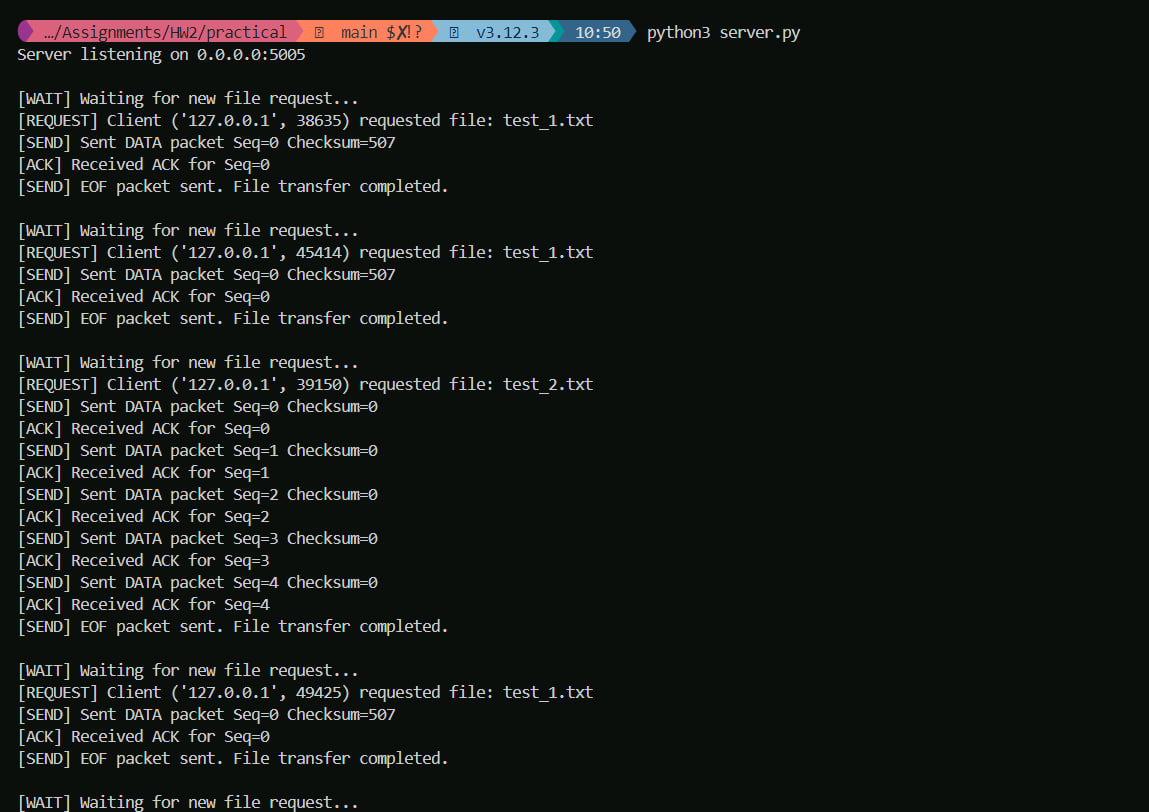
\includegraphics[width=0.7\linewidth]{figs/1}
		
	}
	}


لاگ‌های مرتبط با فایل تست:


		{\centering{
				
				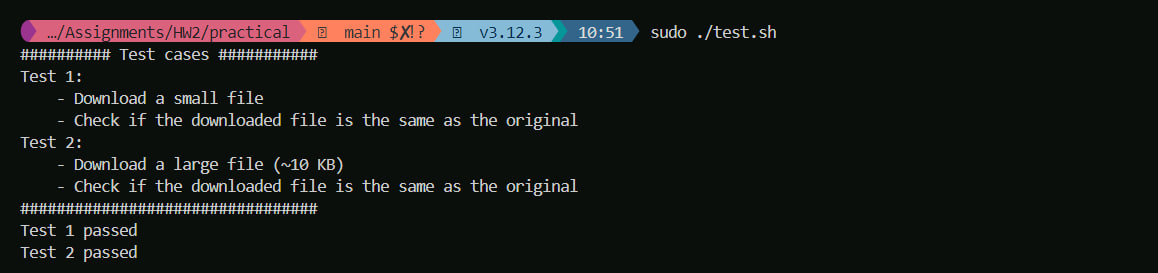
\includegraphics[width=0.7\linewidth]{figs/2}
				
		}}



من برای شبیه‌سازی از دست رفتن بسته‌ها و لینک غیرقابل‌اتکا، داخل کد کلاینت و سرور یک احتمال ثابتی دخیل کردم تا پکت‌ها به مشکل بخورند. سپس آن را روی یک فایل بزرگ‌‌‌تر تست کردم و پکت‌‌های Drop را بررسی کردم که به درستی کار کنند:


{\centering 

{
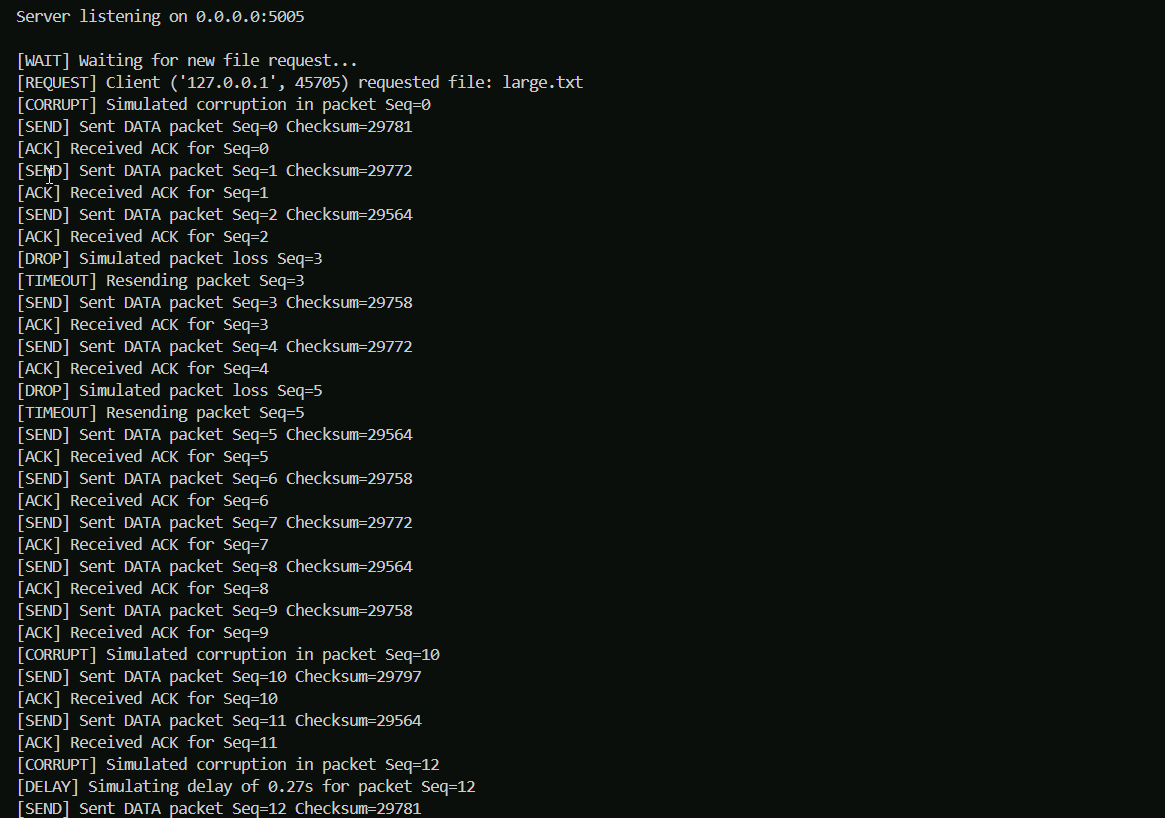
\includegraphics[width=0.7\linewidth]{screenshot001}

}}

همانطور که مشخص است، بعضی از بسته‌ها Drop شده‌اند و seq افزایش نیافته‌است و مجدد ارسال شده است.

همچنین برخی از بسته‌ها Timeout شده‌اند که در عکس لاگ سرور مشخص است. 
در نهایت فایل $large.txt$ به درستی و کامل برای client ارسال شده‌است.


\pagebreak



\pagebreak
\end{document}